\documentclass[11pt,a4paper]{article}
\usepackage{fontspec}
\setmainfont{Latin Modern Roman}
\setmonofont{Latin Modern Mono}[Scale=0.9]
\usepackage[turkish,shorthands=off]{babel}
\usepackage[left=17mm,right=17mm,top=18mm,bottom=18mm,headheight=13pt,headsep=5mm,footskip=9mm]{geometry}
\usepackage{microtype,booktabs,tabularx,array,fancyhdr,lastpage,fvextra}
\usepackage{tikz}
\usetikzlibrary{arrows.meta}
\definecolor{diagramline}{HTML}{B9C3CD}
\definecolor{diagramink}{HTML}{222B35}
\definecolor{diagramarrow}{HTML}{465C74}
\usepackage[hidelinks,unicode]{hyperref}
\hypersetup{pdftitle={Güvenli Kodlama · İlk 7 Hafta · Kavramlar ve Kısaltmalar},pdfauthor={},pdflang={tr-TR}}
\setlength{\parindent}{0pt}
\setlength{\parskip}{4pt}
\setlength{\emergencystretch}{2em}
\renewcommand{\arraystretch}{1.13}
\setlength{\tabcolsep}{5pt}
\newcolumntype{L}{>{\raggedright\arraybackslash}p{.255\linewidth}}
\newcolumntype{Y}{>{\raggedright\arraybackslash}X}
\pagestyle{fancy}\fancyhf{}
\fancyhead[L]{\footnotesize Güvenli Kodlama ve Programlama}
\fancyhead[R]{\footnotesize Kavramlar ve Kısaltmalar · Hafta 1–7}
\fancyfoot[R]{\footnotesize\thepage\,/\,\pageref*{LastPage}}
\newcommand{\AltBaslik}[1]{\par\vspace{3pt}\textbf{#1}\par\nobreak}
\begin{document}
{\Large\bfseries 1 · Güvenlik temelleri}\\[3pt]
{\normalsize Zafiyet, tehdit modeli ve güvenli tasarım}\\[5pt]
\begingroup\small\begin{tabularx}{\linewidth}{@{}LY@{}}\toprule
Kavram & Anlamı ve sınırı\\\midrule
Hata · Zafiyet · İstismar & Bug (hata): yazılımın beklenen davranıştan sapması. Vulnerability (zafiyet): güvenlik etkisi doğuran zayıflık. Exploit (istismar): zafiyeti kullanma yöntemi veya kodu.\\[2pt]
Tehdit · Risk · Etki & Threat (tehdit): zarara yol açabilecek durum veya eylem. Risk: kayıp olasılığı ve etkisinin değerlendirilmesi. Impact (etki): gerçekleşen olayın zararı.\\[2pt]
Saldırı yüzeyi / Attack surface · Güven sınırı / Trust boundary & Erişilebilen girişler / farklı güven düzeyleri arasındaki geçiş. Veri sınırı aşınca yeni bağlamda denetlenir.\\[2pt]
CIA & Confidentiality (gizlilik), Integrity (bütünlük), Availability (kullanılabilirlik).\\[2pt]
CVE / CWE / CVSS & Common Vulnerabilities and Exposures (Yaygın Zafiyetler ve Maruziyetler): zafiyet kaydı. Common Weakness Enumeration (Yaygın Zayıflık Sınıflandırması): zayıflık türü. Common Vulnerability Scoring System (Yaygın Zafiyet Puanlama Sistemi): teknik şiddet puanı.\\[2pt]
CTF · Bayrağı yakala & Capture The Flag: izinli ortamda güvenlik görevleri.\\[2pt]
\bottomrule\end{tabularx}\endgroup\par
\AltBaslik{Kod incelerken}
Girdinin kaynağını, ulaştığı kaynağı ve güven sınırını belirle. Hatalı varsayımı, güvenlik etkisini ve düzeltmeyi göster; aynı denemeyi düzeltmeden sonra tekrarla.

\begingroup\small\begin{tabularx}{\linewidth}{@{}LY@{}}\toprule
İlke & Uygulamadaki karşılığı\\\midrule
Least privilege · en az yetki & Uygulama ve servis hesabı yalnız gereken kaynaklara erişir.\\[2pt]
Fail-safe defaults · güvenli varsayılan & İzin açıkça tanımlı değilse erişim reddedilir.\\[2pt]
Complete mediation · tam denetim & Önemli her erişimde karar yeniden uygulanır. Arayüzde düğmeyi gizlemek yeterli olmaz.\\[2pt]
Defense in depth · katmanlı savunma & Bir kontrol aşılırsa diğerleri etkiyi sınırlayabilir. Ağ kontrolü, uygulamadaki zafiyeti düzeltmez.\\[2pt]
Open design · açık tasarım & Güvenlik algoritmanın gizli kalmasına dayanmaz; anahtarlar korunur.\\[2pt]
\bottomrule\end{tabularx}\endgroup\par
\AltBaslik{STRIDE · Tehdit modelleme / Threat modeling}
\par\noindent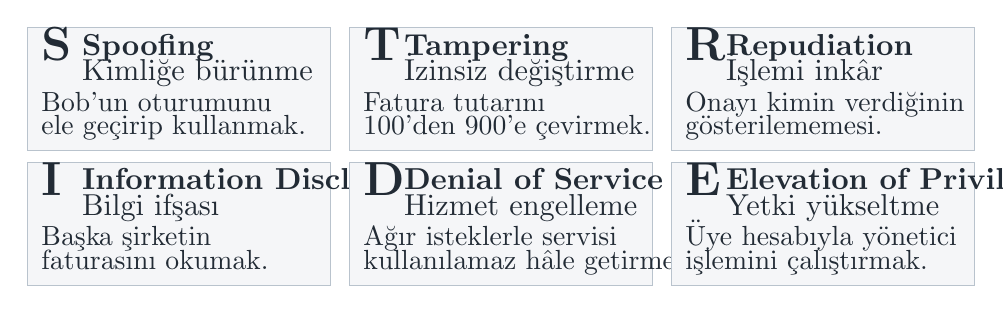
\begin{tikzpicture}[x=.00099\linewidth,y=-.00099\linewidth]
\path[use as bounding box] (0,0) rectangle (1000,274);
\definecolor{vF5F6F8}{HTML}{F5F6F8}
\draw[draw=diagramline,line width=.4pt,fill=vF5F6F8] (0,0) rectangle (320,130);
\node[anchor=base west,inner sep=0pt,text=diagramink,font=\fontsize{16.46}{18.93}\selectfont\bfseries] at (14,35) {S};
\node[anchor=base west,inner sep=0pt,text=diagramink,font=\fontsize{10.48}{12.05}\selectfont\bfseries] at (57,29) {Spoofing};
\node[anchor=base west,inner sep=0pt,text=diagramink,font=\fontsize{10.48}{12.05}\selectfont] at (57,56) {Kimliğe bürünme};
\node[anchor=base west,inner sep=0pt,text=diagramink,font=\fontsize{9.98}{11.48}\selectfont] at (14,88) {Bob’un oturumunu};
\node[anchor=base west,inner sep=0pt,text=diagramink,font=\fontsize{9.98}{11.48}\selectfont] at (14,113) {ele geçirip kullanmak.};
\draw[draw=diagramline,line width=.4pt,fill=vF5F6F8] (340,0) rectangle (660,130);
\node[anchor=base west,inner sep=0pt,text=diagramink,font=\fontsize{16.46}{18.93}\selectfont\bfseries] at (354,35) {T};
\node[anchor=base west,inner sep=0pt,text=diagramink,font=\fontsize{10.48}{12.05}\selectfont\bfseries] at (397,29) {Tampering};
\node[anchor=base west,inner sep=0pt,text=diagramink,font=\fontsize{10.48}{12.05}\selectfont] at (397,56) {İzinsiz değiştirme};
\node[anchor=base west,inner sep=0pt,text=diagramink,font=\fontsize{9.98}{11.48}\selectfont] at (354,88) {Fatura tutarını};
\node[anchor=base west,inner sep=0pt,text=diagramink,font=\fontsize{9.98}{11.48}\selectfont] at (354,113) {100’den 900’e çevirmek.};
\draw[draw=diagramline,line width=.4pt,fill=vF5F6F8] (680,0) rectangle (1000,130);
\node[anchor=base west,inner sep=0pt,text=diagramink,font=\fontsize{16.46}{18.93}\selectfont\bfseries] at (694,35) {R};
\node[anchor=base west,inner sep=0pt,text=diagramink,font=\fontsize{10.48}{12.05}\selectfont\bfseries] at (737,29) {Repudiation};
\node[anchor=base west,inner sep=0pt,text=diagramink,font=\fontsize{10.48}{12.05}\selectfont] at (737,56) {İşlemi inkâr};
\node[anchor=base west,inner sep=0pt,text=diagramink,font=\fontsize{9.98}{11.48}\selectfont] at (694,88) {Onayı kimin verdiğinin};
\node[anchor=base west,inner sep=0pt,text=diagramink,font=\fontsize{9.98}{11.48}\selectfont] at (694,113) {gösterilememesi.};
\draw[draw=diagramline,line width=.4pt,fill=vF5F6F8] (0,142) rectangle (320,272);
\node[anchor=base west,inner sep=0pt,text=diagramink,font=\fontsize{16.46}{18.93}\selectfont\bfseries] at (14,177) {I};
\node[anchor=base west,inner sep=0pt,text=diagramink,font=\fontsize{10.48}{12.05}\selectfont\bfseries] at (57,171) {Information Disclosure};
\node[anchor=base west,inner sep=0pt,text=diagramink,font=\fontsize{10.48}{12.05}\selectfont] at (57,198) {Bilgi ifşası};
\node[anchor=base west,inner sep=0pt,text=diagramink,font=\fontsize{9.98}{11.48}\selectfont] at (14,230) {Başka şirketin};
\node[anchor=base west,inner sep=0pt,text=diagramink,font=\fontsize{9.98}{11.48}\selectfont] at (14,255) {faturasını okumak.};
\draw[draw=diagramline,line width=.4pt,fill=vF5F6F8] (340,142) rectangle (660,272);
\node[anchor=base west,inner sep=0pt,text=diagramink,font=\fontsize{16.46}{18.93}\selectfont\bfseries] at (354,177) {D};
\node[anchor=base west,inner sep=0pt,text=diagramink,font=\fontsize{10.48}{12.05}\selectfont\bfseries] at (397,171) {Denial of Service};
\node[anchor=base west,inner sep=0pt,text=diagramink,font=\fontsize{10.48}{12.05}\selectfont] at (397,198) {Hizmet engelleme};
\node[anchor=base west,inner sep=0pt,text=diagramink,font=\fontsize{9.98}{11.48}\selectfont] at (354,230) {Ağır isteklerle servisi};
\node[anchor=base west,inner sep=0pt,text=diagramink,font=\fontsize{9.98}{11.48}\selectfont] at (354,255) {kullanılamaz hâle getirmek.};
\draw[draw=diagramline,line width=.4pt,fill=vF5F6F8] (680,142) rectangle (1000,272);
\node[anchor=base west,inner sep=0pt,text=diagramink,font=\fontsize{16.46}{18.93}\selectfont\bfseries] at (694,177) {E};
\node[anchor=base west,inner sep=0pt,text=diagramink,font=\fontsize{10.48}{12.05}\selectfont\bfseries] at (737,171) {Elevation of Privilege};
\node[anchor=base west,inner sep=0pt,text=diagramink,font=\fontsize{10.48}{12.05}\selectfont] at (737,198) {Yetki yükseltme};
\node[anchor=base west,inner sep=0pt,text=diagramink,font=\fontsize{9.98}{11.48}\selectfont] at (694,230) {Üye hesabıyla yönetici};
\node[anchor=base west,inner sep=0pt,text=diagramink,font=\fontsize{9.98}{11.48}\selectfont] at (694,255) {işlemini çalıştırmak.};\end{tikzpicture}\par

\newpage
{\Large\bfseries 2 · Injection ve dosya yolları}\\[3pt]
{\normalsize Enjeksiyon / Injection · Dizin dışına çıkma / Path traversal}\\[5pt]
\begingroup\small\begin{tabularx}{\linewidth}{@{}LY@{}}\toprule
Terim / açılım & Nerede ortaya çıkar? · Temel kontrol\\\midrule
SQLi · SQL enjeksiyonu / SQL Injection & Girdi, SQL (Structured Query Language · Yapılandırılmış Sorgu Dili) sorgusunun yapısını değiştirir. Değerler parametreyle; sütun gibi yapısal seçimler izin listesiyle verilir.\\[2pt]
Komut enjeksiyonu / Command injection & \texttt{name=alice; echo DEMO} shell metnine eklenirse ikinci komut çalışabilir. Sabit programı ayrı argümanlarla çağır: \texttt{subprocess.run(["/usr/bin/echo", "Hello", name])}.\\[2pt]
Argüman enjeksiyonu / Argument injection & Girdi \texttt{--help} gibi bir program seçeneği olabilir. Argüman listesi shell’i kaldırır; programın seçenek kuralları ayrıca denetlenir.\\[2pt]
Dizin dışına çıkma / Path traversal & \texttt{../} ile izin verilen klasörün dışına ulaşma. Dosya açmadan önce çözümlenen yolun izinli kök içinde kaldığını denetle.\\[2pt]
LFI · Yerel dosya dahil etme / Local File Inclusion & Sunucudaki bir dosyanın denetimsiz biçimde uygulamaya dahil edilmesi. Dosya içeriği yanıta sızabilir; içerik ve yorumlayıcıya göre kod da çalışabilir.\\[2pt]
\bottomrule\end{tabularx}\endgroup\par
\AltBaslik{SQLi: aynı sorgu, değişen koşul / Changed query condition}
Örnek tablo: \texttt{users} içinde \texttt{(1, Alice)} ve \texttt{(2, Bob)} var. Aşağıdaki değer URL’den çözümlenmiş \texttt{id} parametresidir.

\par\noindent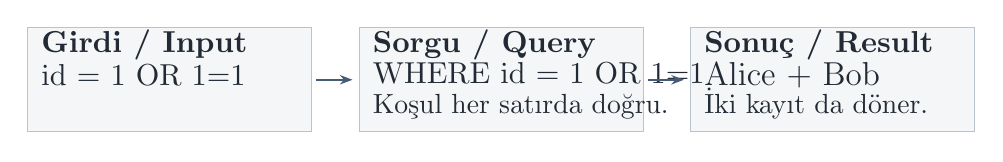
\begin{tikzpicture}[x=.00099\linewidth,y=-.00099\linewidth]
\path[use as bounding box] (0,0) rectangle (1000,112);
\definecolor{vF5F6F8}{HTML}{F5F6F8}
\draw[draw=diagramline,line width=.4pt,fill=vF5F6F8] (0,0) rectangle (300,110);
\draw[draw=diagramline,line width=.4pt,fill=vF5F6F8] (350,0) rectangle (650,110);
\draw[draw=diagramline,line width=.4pt,fill=vF5F6F8] (700,0) rectangle (1000,110);
\node[anchor=base west,inner sep=0pt,text=diagramink,font=\fontsize{10.98}{12.63}\selectfont\bfseries] at (14,26) {Girdi / Input};
\node[anchor=base west,inner sep=0pt,text=diagramink,font=\fontsize{11.47}{13.19}\selectfont] at (14,61) {id = 1 OR 1=1};
\node[anchor=base west,inner sep=0pt,text=diagramink,font=\fontsize{10.98}{12.63}\selectfont\bfseries] at (364,26) {Sorgu / Query};
\node[anchor=base west,inner sep=0pt,text=diagramink,font=\fontsize{10.98}{12.63}\selectfont] at (364,59) {WHERE id = 1 OR 1=1};
\node[anchor=base west,inner sep=0pt,text=diagramink,font=\fontsize{9.98}{11.48}\selectfont] at (364,91) {Koşul her satırda doğru.};
\node[anchor=base west,inner sep=0pt,text=diagramink,font=\fontsize{10.98}{12.63}\selectfont\bfseries] at (714,26) {Sonuç / Result};
\node[anchor=base west,inner sep=0pt,text=diagramink,font=\fontsize{11.97}{13.77}\selectfont] at (714,61) {Alice + Bob};
\node[anchor=base west,inner sep=0pt,text=diagramink,font=\fontsize{9.98}{11.48}\selectfont] at (714,91) {İki kayıt da döner.};
\draw[-{Stealth[length=1.6mm]},draw=diagramarrow,line width=.6pt] (305,55) -- (343,55);
\draw[-{Stealth[length=1.6mm]},draw=diagramarrow,line width=.6pt] (655,55) -- (693,55);\end{tikzpicture}\par
\begin{Verbatim}[fontsize=\footnotesize,breaklines=true,breakanywhere=true,frame=lines,framesep=3mm]
# Hatalı / Vulnerable: girdi sorgu metnine ekleniyor.
q = "SELECT name FROM users WHERE id = " + user_id
# Güvenli / Safe: aynı girdi tek bir değer olarak bağlanıyor.
rows = db.execute("SELECT name FROM users WHERE id = ?", (user_id,))
\end{Verbatim}
Parametreli sürümde \texttt{1 OR 1=1}, SQL operatörü olmaz; bu örnekte hiçbir kullanıcı kimliğiyle eşleşmez.

\AltBaslik{LFI: sayfa seçimi dosya yoluna dönüşür / File inclusion}
\begin{Verbatim}[fontsize=\footnotesize,breaklines=true,breakanywhere=true,frame=lines,framesep=3mm]
// Hatalı PHP örneği / Vulnerable PHP example: view.php
include(__DIR__ . "/pages/" . $_GET["page"]);
// İstek / Request: /view.php?page=../private/note.txt
\end{Verbatim}
\par\noindent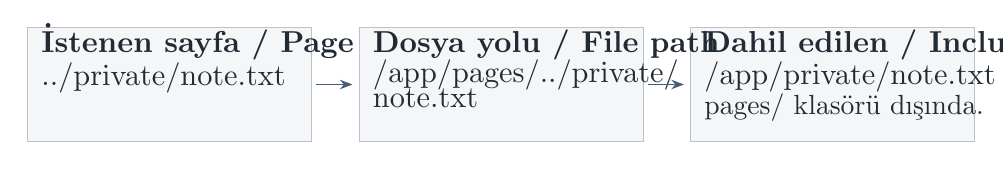
\begin{tikzpicture}[x=.00099\linewidth,y=-.00099\linewidth]
\path[use as bounding box] (0,0) rectangle (1000,122);
\definecolor{vF5F6F8}{HTML}{F5F6F8}
\draw[draw=diagramline,line width=.4pt,fill=vF5F6F8] (0,0) rectangle (300,120);
\draw[draw=diagramline,line width=.4pt,fill=vF5F6F8] (350,0) rectangle (650,120);
\draw[draw=diagramline,line width=.4pt,fill=vF5F6F8] (700,0) rectangle (1000,120);
\node[anchor=base west,inner sep=0pt,text=diagramink,font=\fontsize{10.98}{12.63}\selectfont\bfseries] at (14,26) {İstenen sayfa / Page};
\node[anchor=base west,inner sep=0pt,text=diagramink,font=\fontsize{10.98}{12.63}\selectfont] at (14,61) {../private/note.txt};
\node[anchor=base west,inner sep=0pt,text=diagramink,font=\fontsize{10.98}{12.63}\selectfont\bfseries] at (364,26) {Dosya yolu / File path};
\node[anchor=base west,inner sep=0pt,text=diagramink,font=\fontsize{10.48}{12.05}\selectfont] at (364,58) {/app/pages/../private/};
\node[anchor=base west,inner sep=0pt,text=diagramink,font=\fontsize{10.48}{12.05}\selectfont] at (364,84) {note.txt};
\node[anchor=base west,inner sep=0pt,text=diagramink,font=\fontsize{10.98}{12.63}\selectfont\bfseries] at (714,26) {Dahil edilen / Included};
\node[anchor=base west,inner sep=0pt,text=diagramink,font=\fontsize{10.48}{12.05}\selectfont] at (714,60) {/app/private/note.txt};
\node[anchor=base west,inner sep=0pt,text=diagramink,font=\fontsize{9.98}{11.48}\selectfont] at (714,92) {pages/ klasörü dışında.};
\draw[-{Stealth[length=1.6mm]},draw=diagramarrow,line width=.6pt] (305,60) -- (343,60);
\draw[-{Stealth[length=1.6mm]},draw=diagramarrow,line width=.6pt] (655,60) -- (693,60);\end{tikzpicture}\par
Örnekte \texttt{note.txt} düz metindir; içeriği yanıta eklenir. Düzeltme: kullanıcıdan dosya yolu alma; \texttt{help} gibi bir anahtarı önceden tanımlı dosyaya eşleştir. Tanımsız anahtarı reddet. Bu senaryoda path traversal, LFI’nin izinli klasör dışına ulaşmasını sağlar.


\newpage
{\Large\bfseries 3 · HTTP, tarayıcı ve oturum}\\[3pt]
{\normalsize İstek / Request · Yanıt / Response · Çerez / Cookie}\\[5pt]
\begingroup\small\begin{tabularx}{\linewidth}{@{}LY@{}}\toprule
Terim / açılım & Hatırlanacak nokta\\\midrule
HTTP / HTTPS / TLS & Hypertext Transfer Protocol (Hiper Metin Aktarım Protokolü) / HTTP over TLS (TLS üzerinden HTTP) / Transport Layer Security (Taşıma Katmanı Güvenliği).\\[2pt]
Adres / URL · Köken / Origin · Site & Uniform Resource Locator (Birörnek Kaynak Konumlayıcı). Origin = scheme (şema) + host (sunucu adı) + port. Aynı site içindeki iki alt alan farklı origin olabilir.\\[2pt]
Çerez / Cookie · Oturum / Session & Çerez tarayıcıda tutulan ve kapsamına göre gönderilen veridir. Oturum kaydı sunucuda veya imzalı çerezde olabilir. İmzalı veri, şifreli veri anlamına gelmez.\\[2pt]
Web depolama / Web storage & localStorage (yerel depolama) ve sessionStorage (sekme oturumuna bağlı depolama) JavaScript’ten okunabilir; HTTP isteğine otomatik eklenmez.\\[2pt]
XSS · Siteler arası betik çalıştırma / Cross-Site Scripting & Girdi tarayıcıda kod olarak çalışır. Reflected (yansıtılan): yanıta eklenir. Stored (kalıcı): saklanır, sonraki ziyaretçide çalışır. Metin için \texttt{textContent}; HTML çıktısında bağlama uygun kodlama kullanılır.\\[2pt]
\bottomrule\end{tabularx}\endgroup\par
\AltBaslik{HTTP çerez bayrakları ve öznitelikleri / Cookie flags and attributes}
\begin{Verbatim}[fontsize=\footnotesize,breaklines=true,breakanywhere=true,frame=lines,framesep=3mm]
Set-Cookie: sid=abc123; Secure; HttpOnly; SameSite=Lax
\end{Verbatim}
\begingroup\small\begin{tabularx}{\linewidth}{@{}LY@{}}\toprule
Bayrak / öznitelik & Tarayıcının uyguladığı kural\\\midrule
Secure · Güvenli aktarım bayrağı & Çerez güvenli bağlantıda (genellikle HTTPS) gönderilir. Çerezin içeriğini ayrıca şifrelemez.\\[2pt]
HttpOnly · Betik erişimi kısıtı & \texttt{document.cookie} gibi JavaScript API’leri çerezi okuyamaz. Tarayıcı uygun isteklere çerezi yine ekler.\\[2pt]
SameSite · Siteler arası gönderim & Strict: yalnız aynı site bağlamı. Lax: buna ek olarak üst düzey, güvenli metotlu gezinmeler. None: siteler arası gönderime izin verir; Secure gerekir.\\[2pt]
\bottomrule\end{tabularx}\endgroup\par
\AltBaslik{HTTP durum kodları / HTTP status codes}
\par\noindent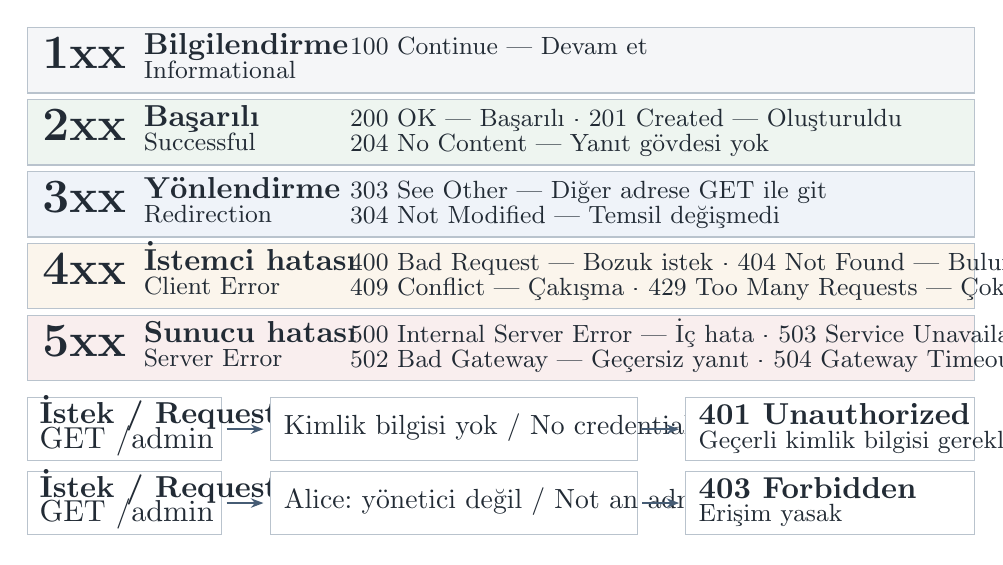
\begin{tikzpicture}[x=.00099\linewidth,y=-.00099\linewidth]
\path[use as bounding box] (0,0) rectangle (1000,538);
\definecolor{vF5F6F8}{HTML}{F5F6F8}
\definecolor{vEEF5F0}{HTML}{EEF5F0}
\definecolor{vFBF5EC}{HTML}{FBF5EC}
\definecolor{vFFFFFF}{HTML}{FFFFFF}
\definecolor{vEFF3F9}{HTML}{EFF3F9}
\definecolor{vF9EEEE}{HTML}{F9EEEE}
\draw[draw=diagramline,line width=.4pt,fill=vF5F6F8] (0,0) rectangle (1000,69);
\node[anchor=base west,inner sep=0pt,text=diagramink,font=\fontsize{15.96}{18.35}\selectfont\bfseries] at (15,43) {1xx};
\node[anchor=base west,inner sep=0pt,text=diagramink,font=\fontsize{10.48}{12.05}\selectfont\bfseries] at (122,28) {Bilgilendirme};
\node[anchor=base west,inner sep=0pt,text=diagramink,font=\fontsize{9.48}{10.90}\selectfont] at (122,54) {Informational};
\node[anchor=base west,inner sep=0pt,text=diagramink,font=\fontsize{8.98}{10.33}\selectfont] at (340,28) {100 Continue — Devam et};
\draw[draw=diagramline,line width=.4pt,fill=vEEF5F0] (0,76) rectangle (1000,145);
\node[anchor=base west,inner sep=0pt,text=diagramink,font=\fontsize{15.96}{18.35}\selectfont\bfseries] at (15,119) {2xx};
\node[anchor=base west,inner sep=0pt,text=diagramink,font=\fontsize{10.48}{12.05}\selectfont\bfseries] at (122,104) {Başarılı};
\node[anchor=base west,inner sep=0pt,text=diagramink,font=\fontsize{9.48}{10.90}\selectfont] at (122,130) {Successful};
\node[anchor=base west,inner sep=0pt,text=diagramink,font=\fontsize{8.98}{10.33}\selectfont] at (340,104) {200 OK — Başarılı · 201 Created — Oluşturuldu};
\node[anchor=base west,inner sep=0pt,text=diagramink,font=\fontsize{8.98}{10.33}\selectfont] at (340,131) {204 No Content — Yanıt gövdesi yok};
\draw[draw=diagramline,line width=.4pt,fill=vEFF3F9] (0,152) rectangle (1000,221);
\node[anchor=base west,inner sep=0pt,text=diagramink,font=\fontsize{15.96}{18.35}\selectfont\bfseries] at (15,195) {3xx};
\node[anchor=base west,inner sep=0pt,text=diagramink,font=\fontsize{10.48}{12.05}\selectfont\bfseries] at (122,180) {Yönlendirme};
\node[anchor=base west,inner sep=0pt,text=diagramink,font=\fontsize{9.48}{10.90}\selectfont] at (122,206) {Redirection};
\node[anchor=base west,inner sep=0pt,text=diagramink,font=\fontsize{8.98}{10.33}\selectfont] at (340,180) {303 See Other — Diğer adrese GET ile git};
\node[anchor=base west,inner sep=0pt,text=diagramink,font=\fontsize{8.98}{10.33}\selectfont] at (340,207) {304 Not Modified — Temsil değişmedi};
\draw[draw=diagramline,line width=.4pt,fill=vFBF5EC] (0,228) rectangle (1000,297);
\node[anchor=base west,inner sep=0pt,text=diagramink,font=\fontsize{15.96}{18.35}\selectfont\bfseries] at (15,271) {4xx};
\node[anchor=base west,inner sep=0pt,text=diagramink,font=\fontsize{10.48}{12.05}\selectfont\bfseries] at (122,256) {İstemci hatası};
\node[anchor=base west,inner sep=0pt,text=diagramink,font=\fontsize{9.48}{10.90}\selectfont] at (122,282) {Client Error};
\node[anchor=base west,inner sep=0pt,text=diagramink,font=\fontsize{8.98}{10.33}\selectfont] at (340,256) {400 Bad Request — Bozuk istek · 404 Not Found — Bulunamadı};
\node[anchor=base west,inner sep=0pt,text=diagramink,font=\fontsize{8.98}{10.33}\selectfont] at (340,283) {409 Conflict — Çakışma · 429 Too Many Requests — Çok fazla istek};
\draw[draw=diagramline,line width=.4pt,fill=vF9EEEE] (0,304) rectangle (1000,373);
\node[anchor=base west,inner sep=0pt,text=diagramink,font=\fontsize{15.96}{18.35}\selectfont\bfseries] at (15,347) {5xx};
\node[anchor=base west,inner sep=0pt,text=diagramink,font=\fontsize{10.48}{12.05}\selectfont\bfseries] at (122,332) {Sunucu hatası};
\node[anchor=base west,inner sep=0pt,text=diagramink,font=\fontsize{9.48}{10.90}\selectfont] at (122,358) {Server Error};
\node[anchor=base west,inner sep=0pt,text=diagramink,font=\fontsize{8.98}{10.33}\selectfont] at (340,332) {500 Internal Server Error — İç hata · 503 Service Unavailable — Hizmet yok};
\node[anchor=base west,inner sep=0pt,text=diagramink,font=\fontsize{8.98}{10.33}\selectfont] at (340,359) {502 Bad Gateway — Geçersiz yanıt · 504 Gateway Timeout — Zaman aşımı};
\draw[draw=diagramline,line width=.4pt,fill=vFFFFFF] (0,391) rectangle (205,457);
\node[anchor=base west,inner sep=0pt,text=diagramink,font=\fontsize{10.48}{12.05}\selectfont\bfseries] at (12,418) {İstek / Request};
\node[anchor=base west,inner sep=0pt,text=diagramink,font=\fontsize{10.48}{12.05}\selectfont] at (12,444) {GET /admin};
\draw[draw=diagramline,line width=.4pt,fill=vFFFFFF] (256,391) rectangle (644,457);
\node[anchor=base west,inner sep=0pt,text=diagramink,font=\fontsize{9.98}{11.48}\selectfont] at (270,430) {Kimlik bilgisi yok / No credentials};
\draw[draw=diagramline,line width=.4pt,fill=vFFFFFF] (695,391) rectangle (1000,457);
\node[anchor=base west,inner sep=0pt,text=diagramink,font=\fontsize{11.47}{13.19}\selectfont\bfseries] at (708,419) {401 Unauthorized};
\node[anchor=base west,inner sep=0pt,text=diagramink,font=\fontsize{9.48}{10.90}\selectfont] at (708,444) {Geçerli kimlik bilgisi gerekli};
\draw[-{Stealth[length=1.6mm]},draw=diagramarrow,line width=.6pt] (210,424) -- (249,424);
\draw[-{Stealth[length=1.6mm]},draw=diagramarrow,line width=.6pt] (649,424) -- (688,424);
\draw[draw=diagramline,line width=.4pt,fill=vFFFFFF] (0,469) rectangle (205,535);
\node[anchor=base west,inner sep=0pt,text=diagramink,font=\fontsize{10.48}{12.05}\selectfont\bfseries] at (12,496) {İstek / Request};
\node[anchor=base west,inner sep=0pt,text=diagramink,font=\fontsize{10.48}{12.05}\selectfont] at (12,522) {GET /admin};
\draw[draw=diagramline,line width=.4pt,fill=vFFFFFF] (256,469) rectangle (644,535);
\node[anchor=base west,inner sep=0pt,text=diagramink,font=\fontsize{9.98}{11.48}\selectfont] at (270,508) {Alice: yönetici değil / Not an admin};
\draw[draw=diagramline,line width=.4pt,fill=vFFFFFF] (695,469) rectangle (1000,535);
\node[anchor=base west,inner sep=0pt,text=diagramink,font=\fontsize{11.47}{13.19}\selectfont\bfseries] at (708,497) {403 Forbidden};
\node[anchor=base west,inner sep=0pt,text=diagramink,font=\fontsize{9.48}{10.90}\selectfont] at (708,522) {Erişim yasak};
\draw[-{Stealth[length=1.6mm]},draw=diagramarrow,line width=.6pt] (210,502) -- (249,502);
\draw[-{Stealth[length=1.6mm]},draw=diagramarrow,line width=.6pt] (649,502) -- (688,502);\end{tikzpicture}\par

\newpage
{\Large\bfseries 4 · Uygulamalı kriptografi}\\[3pt]
{\normalsize Kodlama, şifreleme, özet ve imza}\\[5pt]
\begingroup\small\begin{tabularx}{\linewidth}{@{}LY@{}}\toprule
Yöntem / açılım & Sağladığı özellik ve dikkat noktası\\\midrule
Kodlama / Encoding · Base64 / Base64url & Gösterimi değiştirir; anahtar (key) gerektirmez. Gizlilik veya bütünlük sağlamaz.\\[2pt]
Simetrik şifreleme / Symmetric encryption · AES & Advanced Encryption Standard (Gelişmiş Şifreleme Standardı). Şifreleme ve çözmede aynı gizli anahtar (secret key) kullanılır.\\[2pt]
Asimetrik yöntemler / Asymmetric methods & Açık anahtar (public key) / özel anahtar (private key) çifti. RSA-OAEP: şifreleme (encryption); Ed25519: imza (signature); Diffie–Hellman ve X25519: anahtar anlaşması (key agreement).\\[2pt]
Özetleme / Hashing · SHA-256 & Secure Hash Algorithm (Güvenli Özet Algoritması), 256 bit. Tek yönlü özet (hash). Güvenilir kaynaktaki özetle karşılaştırma değişikliği saptayabilir.\\[2pt]
HMAC · Anahtarlı mesaj doğrulama & Hash-based Message Authentication Code (Özet Tabanlı Mesaj Doğrulama Kodu). İçeriği gizlemez; aynı anahtarı bilenler doğrulama etiketi (tag) üretebilir.\\[2pt]
Dijital imza / Digital signature & Özel anahtar imzalar, açık anahtar doğrular. Açık anahtarın kime ait olduğu ayrıca belirlenir.\\[2pt]
RNG / PRNG / CSPRNG & Random Number Generator (Rastgele Sayı Üreteci) / Pseudorandom Number Generator (Sözde Rastgele Sayı Üreteci) / Cryptographically Secure PRNG (Kriptografik Olarak Güvenli PRNG). Sabit tohum (seed) ile çalışan \texttt{random}, güvenlik token’ı için uygun değildir.\\[2pt]
Tek kullanımlık değer / Nonce · Tuz / Salt & Nonce: number used once; yöntemin tekrar etmeme kuralına tabi değer. Salt: parola kaydını farklılaştıran değer. Gizli olmaları gerekmez.\\[2pt]
\bottomrule\end{tabularx}\endgroup\par
\AltBaslik{Güvenli rastgelelik ve aday sayısı}
\begin{Verbatim}[fontsize=\footnotesize,breaklines=true,breakanywhere=true,frame=lines,framesep=3mm]
import secrets
reset_token = secrets.token_urlsafe(32)  # 32 bayt rastgelelik
nonce = secrets.token_bytes(12)         # AES-GCM örneği
\end{Verbatim}
Eşit olasılıkla üretilen L uzunluğunda, A sembollü bir değer için aday sayısı N = A\textasciicircum{}L. Sabit deneme hızı r ise tam tarama süresi yaklaşık N/r, rastgele hedefte ortalama yaklaşık yarısıdır. 4 rakamlı PIN’in SHA-256 özeti de yalnız 10.000 PIN adayından biridir.

Gökkuşağı tablosu (rainbow table), özet ve indirgeme (reduction) zincirleriyle ön hesaplama/bellek takası yapar. Salt, aynı ön hesabın bütün kayıtlarda kullanılmasını engeller. Parola için ayrıca Argon2id gibi maliyetli bir parola özetleme yöntemi gerekir.


\newpage
{\Large\bfseries 5 · Parola ve kimlik doğrulama}\\[3pt]
{\normalsize Deneme saldırıları, güvenli saklama ve MFA}\\[5pt]
\begingroup\small\begin{tabularx}{\linewidth}{@{}LY@{}}\toprule
Terim / açılım & Ayırıcı özellik\\\midrule
Kimlik doğrulama / Authentication · Yetkilendirme / Authorization & Hangi hesap olduğunu doğrulamak ve hangi işlem/kaynağa erişebileceğine karar vermek ayrı kontrollerdir.\\[2pt]
Kaba kuvvet / Brute force · Sözlük / Dictionary · Maske / Mask & Aday uzayını tarama / sözlükten aday seçme / bilinen biçime göre aday üretme.\\[2pt]
Parola püskürtme / Password spraying & Çok hesaba az sayıda yaygın parola deneme. Yalnız hesap başına kilit yeterli olmayabilir.\\[2pt]
Çalıntı kimlik bilgisi denemesi / Credential stuffing & Başka hizmetten çalınan kullanıcı adı–parola çiftlerini deneme. Tekrar kullanılmayan parolalar ve MFA etkiyi sınırlar.\\[2pt]
Hesap varlığı tespiti / User enumeration & Mesaj, süre veya yanıt farkıyla hesabın varlığını öğrenme. Tutarlı hata yanıtı ve kontrollü işlem yolu gerekir.\\[2pt]
Çevrim içi / Online · Çevrim dışı / Offline & Giriş noktasında deneme / ele geçmiş özet üzerinde yerel deneme. İstek hızı sınırı (rate limiting), çevrim dışı denemeyi durdurmaz.\\[2pt]
Parola özetleme / Password hashing · Argon2id / bcrypt & Maliyetli parola özetleme yöntemleri. Tuz (salt) ve maliyet (cost) ayarı kayıtta tutulur. Hızlı SHA-256 tek başına parola saklama yöntemi değildir.\\[2pt]
MFA / TOTP & Multi-Factor Authentication (Çok Faktörlü Kimlik Doğrulama) / Time-based One-Time Password (Zaman Tabanlı Tek Kullanımlık Parola). TOTP’de süre ve tekrar kullanım denetlenir.\\[2pt]
\bottomrule\end{tabularx}\endgroup\par
\AltBaslik{Kimlik doğrulama faktörleri / Authentication factors}
\begingroup\small\begin{tabularx}{\linewidth}{@{}LY@{}}\toprule
Faktör / Factor & Örnek / Example\\\midrule
Bildiğin bir şey / Something you know & Parola veya PIN: kullanıcının bildiği bilgi.\\[2pt]
Sahip olduğun bir şey / Something you have & Güvenlik anahtarı veya doğrulama uygulamasının kurulu olduğu telefon: kullanıcının elindeki araç.\\[2pt]
Olduğun bir şey / Something you are & Parmak izi veya yüz gibi biyometrik özellik.\\[2pt]
\bottomrule\end{tabularx}\endgroup\par
MFA, en az iki farklı gruptan faktör kullanır: parola + güvenlik anahtarı gibi. İki ayrı parola aynı gruptadır. Geçiş anahtarında (passkey), cihazda veya güvenlik anahtarında tutulan kriptografik anahtar kullanılır. Cihaz PIN’i veya biyometri bu anahtarı yerel olarak kullanıma açabilir.

\AltBaslik{Uygulamada}
NIST SP 800-63B-4: tek faktörlü parola en az 15 karakter; MFA parçası olduğunda en az 8 karaktere izin verilebilir. Uzun parolalar desteklenir; yaygın/sızmış değerler engellenir. Karakter türü zorlaması ve ihlal belirtisi olmadan dönemsel değişim istenmez. Parola yöneticileri ve yapıştırma desteklenir.

Girişlerde hesap, ağ ve genel trafik bağlamında deneme sınırı; tutarlı hata mesajı; yok hesap için maliyetli doğrulama yolu; başarıdan sonra yeni oturum gerekir. Hesap kilidinin hizmet engellemeye dönüşebileceği de düşünülür.

Parola sıfırlama (password reset): CSPRNG ile üretilmiş token; kullanıcıya bağlı, kısa ömürlü ve tek kullanımlık kayıt. Token loglanmaz. Bilgi hırsızı yazılım (infostealer), parolayı veya hazır oturumu kopyalayabilir; MFA her oturum hırsızlığını önlemez.


\newpage
{\Large\bfseries 6 · Yetkilendirme}\\[3pt]
{\normalsize Tek vaka: aynı faturada kayıt, işlem ve alan izinleri}\\[5pt]
A şirketinde Alice ve Bob üye, Deniz muhasebecidir. Üyeler kendi veya düzenleyici olarak paylaşılan faturaları okur, notlarını değiştirir. Muhasebeci aynı şirketteki, limiti içindeki taslak faturayı onaylayabilir.

\par\noindent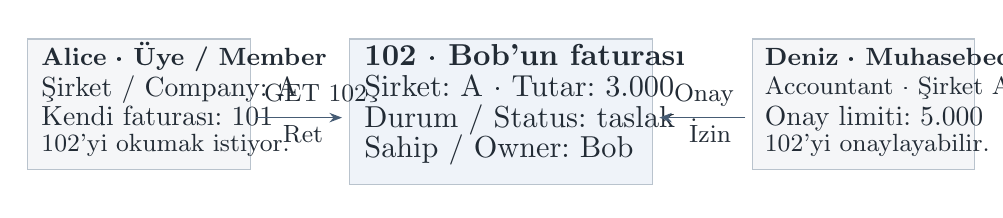
\begin{tikzpicture}[x=.00099\linewidth,y=-.00099\linewidth]
\path[use as bounding box] (0,0) rectangle (1000,171);
\definecolor{vF5F6F8}{HTML}{F5F6F8}
\definecolor{vEFF3F9}{HTML}{EFF3F9}
\draw[draw=diagramline,line width=.4pt,fill=vF5F6F8] (0,12) rectangle (235,150);
\node[anchor=base west,inner sep=0pt,text=diagramink,font=\fontsize{9.48}{10.90}\selectfont\bfseries] at (14,40) {Alice · Üye / Member};
\node[anchor=base west,inner sep=0pt,text=diagramink,font=\fontsize{9.98}{11.48}\selectfont] at (14,73) {Şirket / Company: A};
\node[anchor=base west,inner sep=0pt,text=diagramink,font=\fontsize{9.98}{11.48}\selectfont] at (14,103) {Kendi faturası: 101};
\node[anchor=base west,inner sep=0pt,text=diagramink,font=\fontsize{9.48}{10.90}\selectfont] at (14,131) {102’yi okumak istiyor.};
\draw[draw=diagramline,line width=.4pt,fill=vEFF3F9] (340,12) rectangle (660,166);
\node[anchor=base west,inner sep=0pt,text=diagramink,font=\fontsize{11.47}{13.19}\selectfont\bfseries] at (355,40) {102 · Bob’un faturası};
\node[anchor=base west,inner sep=0pt,text=diagramink,font=\fontsize{10.48}{12.05}\selectfont] at (355,73) {Şirket: A · Tutar: 3.000};
\node[anchor=base west,inner sep=0pt,text=diagramink,font=\fontsize{10.48}{12.05}\selectfont] at (355,105) {Durum / Status: taslak};
\node[anchor=base west,inner sep=0pt,text=diagramink,font=\fontsize{10.48}{12.05}\selectfont] at (355,137) {Sahip / Owner: Bob};
\draw[draw=diagramline,line width=.4pt,fill=vF5F6F8] (765,12) rectangle (1000,150);
\node[anchor=base west,inner sep=0pt,text=diagramink,font=\fontsize{9.48}{10.90}\selectfont\bfseries] at (778,40) {Deniz · Muhasebeci};
\node[anchor=base west,inner sep=0pt,text=diagramink,font=\fontsize{9.48}{10.90}\selectfont] at (778,71) {Accountant · Şirket A};
\node[anchor=base west,inner sep=0pt,text=diagramink,font=\fontsize{9.98}{11.48}\selectfont] at (778,103) {Onay limiti: 5.000};
\node[anchor=base west,inner sep=0pt,text=diagramink,font=\fontsize{9.48}{10.90}\selectfont] at (778,131) {102’yi onaylayabilir.};
\node[anchor=base west,inner sep=0pt,text=diagramink,font=\fontsize{8.98}{10.33}\selectfont] at (249,78) {GET 102};
\draw[-{Stealth[length=1.6mm]},draw=diagramarrow,line width=.6pt] (241,95) -- (332,95);
\node[anchor=base west,inner sep=0pt,text=diagramink,font=\fontsize{8.98}{10.33}\selectfont] at (682,78) {Onay};
\node[anchor=base west,inner sep=0pt,text=diagramink,font=\fontsize{8.98}{10.33}\selectfont] at (269,121) {Ret};
\node[anchor=base west,inner sep=0pt,text=diagramink,font=\fontsize{8.98}{10.33}\selectfont] at (698,121) {İzin};
\draw[-{Stealth[length=1.6mm]},draw=diagramarrow,line width=.6pt] (758,95) -- (667,95);\end{tikzpicture}\par
\begingroup\small\begin{tabularx}{\linewidth}{@{}LY@{}}\toprule
Kontrolün yeri & Aynı vakada ne olur?\\\midrule
IDOR / BOLA & Insecure Direct Object Reference (Güvensiz Doğrudan Nesne Referansı) / Broken Object Level Authorization (Nesne Düzeyinde Yetkilendirme Eksikliği). Alice, \texttt{GET /invoices/101} yerine \texttt{GET /invoices/102} gönderir. İzni yokken Bob’un faturası dönüyorsa nesne erişimi hatalıdır; bu örnekte iki ad aynı sorunun farklı yönlerini anlatır.\\[2pt]
BFLA & Broken Function Level Authorization (İşlev Düzeyinde Yetkilendirme Eksikliği). Alice, \texttt{POST /invoices/101/approve} çağırır. Fatura kendisinin olsa da onay rolü yoktur; işlem reddedilmelidir.\\[2pt]
BOPLA & Broken Object Property Level Authorization (Nesne Alanı Düzeyinde Yetkilendirme Eksikliği). Alice 101’in notunu değiştirebilir; aynı istekte \texttt{status=approved} göndererek faturayı onaylayamaz. Toplu alan atama (mass assignment) bu sınırı aşmamalıdır.\\[2pt]
RBAC & Role-Based Access Control (Rol Tabanlı Erişim Kontrolü). Deniz’in muhasebeci rolü onay işlevine erişim sağlar. Alice’in üyeliği sağlamaz.\\[2pt]
ABAC & Attribute-Based Access Control (Öznitelik Tabanlı Erişim Kontrolü). 102 aynı şirkette, 3.000 tutarı 5.000 limitinin altında ve taslak durumunda: Deniz’in onay koşulları sağlanır.\\[2pt]
ReBAC & Relationship-Based Access Control (İlişki Tabanlı Erişim Kontrolü). Bob, Alice’i 102’ye düzenleyici olarak eklerse Alice notu değiştirebilir. Bu paylaşım onay yetkisi vermez.\\[2pt]
\bottomrule\end{tabularx}\endgroup\par
Her işlem için gereken kontroller birlikte uygulanır. UUID (Universally Unique Identifier · Evrensel Benzersiz Tanımlayıcı) kullanmak bu izinleri sağlamaz. Okuma, not değiştirme ve onay için farklı kararlar verilebilir.


\newpage
\setlength{\parskip}{2pt}\renewcommand{\AltBaslik}[1]{\par\vspace{1pt}\textbf{#1}\par\nobreak}
{\Large\bfseries 7 · JWT, OAuth, SSO ve loglama}\\[3pt]
{\normalsize Token’ın yolculuğu, ortak giriş ve kayıttan alarma}\\[5pt]
\begingroup\small\begin{tabularx}{\linewidth}{@{}LY@{}}\toprule
Kavram / Concept & Kısa karşılığı\\\midrule
JWT / JWS / JWE & JSON Web Token (JSON Web Belirteci); JSON Web Signature (JSON Web İmzası); JSON Web Encryption (JSON Web Şifrelemesi). İmzalı JWT’nin içeriği okunabilir.\\[2pt]
Simetrik / Symmetric · Asimetrik / Asymmetric & HS256: üreten ve doğrulayan hizmet aynı gizli anahtarı bilir. RS256: özel anahtar (private key) imzalar; açık anahtar (public key) doğrular.\\[2pt]
OAuth / OIDC / SSO & OAuth 2.0 Authorization Framework (Yetkilendirme Çerçevesi): API yetkisi. OpenID Connect: kimlik doğrulama. Single Sign-On (Tek Oturum Açma): bir girişle birden çok uygulama.\\[2pt]
Access / ID / Refresh token & Erişim / kimlik / yenileme token’ı: API isteği / giriş sonucu / yeni erişim token’ı alma. ID token API’ye erişim belgesi değildir.\\[2pt]
PKCE / state / nonce & Proof Key for Code Exchange (Kod Değişimi için İspat Anahtarı): kodu istemciye bağlar. State (işlem durumu) dönüşü giriş denemesiyle eşleştirir. Nonce (tek kullanımlık değer), ID token’ı isteğe bağlar.\\[2pt]
iss / sub / aud / exp & Issuer (üretici) / Subject (özne) / Audience (alıcı) / Expiration Time (bitiş zamanı). API imza, üretici, alıcı ve süreyi; sonra nesne/işlem iznini kontrol eder.\\[2pt]
\bottomrule\end{tabularx}\endgroup\par
\AltBaslik{1 · JWT nerede durur? / Token flow}
\par\noindent
\begin{tikzpicture}[x=.00099\linewidth,y=-.00099\linewidth]
\path[use as bounding box] (0,0) rectangle (1000,100);
\definecolor{vF5F6F8}{HTML}{F5F6F8}
\draw[draw=diagramline,line width=.4pt,fill=vF5F6F8] (0,0) rectangle (300,98);
\draw[draw=diagramline,line width=.4pt,fill=vF5F6F8] (350,0) rectangle (650,98);
\draw[draw=diagramline,line width=.4pt,fill=vF5F6F8] (700,0) rectangle (1000,98);
\node[anchor=base west,inner sep=0pt,text=diagramink,font=\fontsize{11.47}{13.19}\selectfont\bfseries] at (14,31) {Sunucu / Server};
\node[anchor=base west,inner sep=0pt,text=diagramink,font=\fontsize{9.98}{11.48}\selectfont] at (14,70) {İmzalı token üretir.};
\node[anchor=base west,inner sep=0pt,text=diagramink,font=\fontsize{11.47}{13.19}\selectfont\bfseries] at (364,31) {İstemci / Client};
\node[anchor=base west,inner sep=0pt,text=diagramink,font=\fontsize{9.98}{11.48}\selectfont] at (364,70) {Token’ı saklar ve taşır.};
\node[anchor=base west,inner sep=0pt,text=diagramink,font=\fontsize{11.47}{13.19}\selectfont\bfseries] at (714,31) {API};
\node[anchor=base west,inner sep=0pt,text=diagramink,font=\fontsize{9.98}{11.48}\selectfont] at (714,70) {İmza, süre ve izin kontrolü.};
\draw[-{Stealth[length=1.6mm]},draw=diagramarrow,line width=.6pt] (305,49) -- (343,49);
\draw[-{Stealth[length=1.6mm]},draw=diagramarrow,line width=.6pt] (655,49) -- (693,49);\end{tikzpicture}\par
Token istemcide saklanıp istekle gönderilir. HttpOnly çerez ve JavaScript depolarının riskleri farklıdır. Gizli/özel anahtar istemciye verilmez. Sunucu gerektiğinde hesap ve iptal kaydı tutar.

\AltBaslik{2 · Kurumsal giriş / Corporate sign-in}
\par\noindent
\begin{tikzpicture}[x=.00099\linewidth,y=-.00099\linewidth]
\path[use as bounding box] (0,0) rectangle (1000,92);
\definecolor{vF5F6F8}{HTML}{F5F6F8}
\draw[draw=diagramline,line width=.4pt,fill=vF5F6F8] (0,0) rectangle (220,90);
\node[anchor=base west,inner sep=0pt,text=diagramink,font=\fontsize{10.48}{12.05}\selectfont\bfseries] at (12,31) {Girişi başlat};
\node[anchor=base west,inner sep=0pt,text=diagramink,font=\fontsize{9.48}{10.90}\selectfont] at (12,67) {Start login};
\draw[-{Stealth[length=1.6mm]},draw=diagramarrow,line width=.6pt] (225,45) -- (253,45);
\draw[draw=diagramline,line width=.4pt,fill=vF5F6F8] (260,0) rectangle (480,90);
\node[anchor=base west,inner sep=0pt,text=diagramink,font=\fontsize{10.48}{12.05}\selectfont\bfseries] at (272,31) {Kimliği doğrula};
\node[anchor=base west,inner sep=0pt,text=diagramink,font=\fontsize{9.48}{10.90}\selectfont] at (272,67) {Authenticate};
\draw[-{Stealth[length=1.6mm]},draw=diagramarrow,line width=.6pt] (485,45) -- (513,45);
\draw[draw=diagramline,line width=.4pt,fill=vF5F6F8] (520,0) rectangle (740,90);
\node[anchor=base west,inner sep=0pt,text=diagramink,font=\fontsize{10.48}{12.05}\selectfont\bfseries] at (532,31) {Dönüşü denetle};
\node[anchor=base west,inner sep=0pt,text=diagramink,font=\fontsize{9.48}{10.90}\selectfont] at (532,67) {Validate return};
\draw[-{Stealth[length=1.6mm]},draw=diagramarrow,line width=.6pt] (745,45) -- (773,45);
\draw[draw=diagramline,line width=.4pt,fill=vF5F6F8] (780,0) rectangle (1000,90);
\node[anchor=base west,inner sep=0pt,text=diagramink,font=\fontsize{10.48}{12.05}\selectfont\bfseries] at (792,31) {Oturum aç};
\node[anchor=base west,inner sep=0pt,text=diagramink,font=\fontsize{9.48}{10.90}\selectfont] at (792,67) {App session};\end{tikzpicture}\par
Uygulama dönüşü doğrular ve kendi oturumunu açar. SSO’da ortak giriş hizmetinin açık oturumu ikinci uygulamada da kullanılabilir; uygulamaların yerel oturumları ayrıdır.

\AltBaslik{3 · Kayıttan alarma / Logs to alerts}
\par\noindent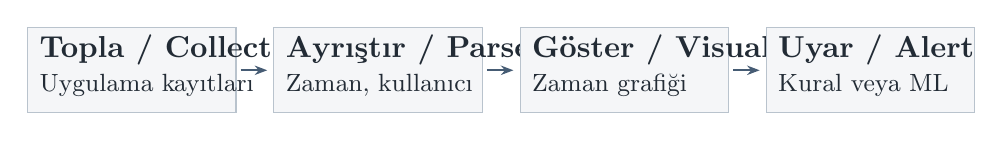
\begin{tikzpicture}[x=.00099\linewidth,y=-.00099\linewidth]
\path[use as bounding box] (0,0) rectangle (1000,92);
\definecolor{vF5F6F8}{HTML}{F5F6F8}
\draw[draw=diagramline,line width=.4pt,fill=vF5F6F8] (0,0) rectangle (220,90);
\node[anchor=base west,inner sep=0pt,text=diagramink,font=\fontsize{10.48}{12.05}\selectfont\bfseries] at (12,31) {Topla / Collect};
\node[anchor=base west,inner sep=0pt,text=diagramink,font=\fontsize{9.48}{10.90}\selectfont] at (12,67) {Uygulama kayıtları};
\draw[-{Stealth[length=1.6mm]},draw=diagramarrow,line width=.6pt] (225,45) -- (253,45);
\draw[draw=diagramline,line width=.4pt,fill=vF5F6F8] (260,0) rectangle (480,90);
\node[anchor=base west,inner sep=0pt,text=diagramink,font=\fontsize{10.48}{12.05}\selectfont\bfseries] at (272,31) {Ayrıştır / Parse};
\node[anchor=base west,inner sep=0pt,text=diagramink,font=\fontsize{9.48}{10.90}\selectfont] at (272,67) {Zaman, kullanıcı};
\draw[-{Stealth[length=1.6mm]},draw=diagramarrow,line width=.6pt] (485,45) -- (513,45);
\draw[draw=diagramline,line width=.4pt,fill=vF5F6F8] (520,0) rectangle (740,90);
\node[anchor=base west,inner sep=0pt,text=diagramink,font=\fontsize{10.48}{12.05}\selectfont\bfseries] at (532,31) {Göster / Visualize};
\node[anchor=base west,inner sep=0pt,text=diagramink,font=\fontsize{9.48}{10.90}\selectfont] at (532,67) {Zaman grafiği};
\draw[-{Stealth[length=1.6mm]},draw=diagramarrow,line width=.6pt] (745,45) -- (773,45);
\draw[draw=diagramline,line width=.4pt,fill=vF5F6F8] (780,0) rectangle (1000,90);
\node[anchor=base west,inner sep=0pt,text=diagramink,font=\fontsize{10.48}{12.05}\selectfont\bfseries] at (792,31) {Uyar / Alert};
\node[anchor=base west,inner sep=0pt,text=diagramink,font=\fontsize{9.48}{10.90}\selectfont] at (792,67) {Kural veya ML};\end{tikzpicture}\par
Data parsing (veri ayrıştırma) alanları çıkarır; data visualization (veri görselleştirme) örüntüyü gösterir. ML (Machine Learning · Makine öğrenmesi), olağan düzenden sapmaları işaretleyebilir. Anomaly detection (anomali tespiti), inceleme sinyalidir; her sapma saldırı değildir.

Logda zaman, doğrulanmış kullanıcı, kaynak, sonuç ve istek kimliği bulunur. DEBUG (hata ayıklama), INFO (bilgi), WARNING (uyarı), ERROR (hata). Parola, çerez ve token kaydedilmez.

\AltBaslik{Dosya yükleme / File upload}
Örnek: Görsel ekinde \texttt{Content-Type: image/jpeg} (içerik türü) yazması, dosyanın görsel olduğunu kanıtlamaz. Tür, içerik ve boyut sunucuda denetlenir. Dosya sunucunun verdiği adla web kökü dışında saklanır; yükleme ve indirmede izin aranır.

\AltBaslik{RCE · Uzaktan kod çalıştırma / Remote Code Execution}
\par\noindent
\begin{tikzpicture}[x=.00099\linewidth,y=-.00099\linewidth]
\path[use as bounding box] (0,0) rectangle (1000,56);
\definecolor{vF5F6F8}{HTML}{F5F6F8}
\draw[draw=diagramline,line width=.4pt,fill=vF5F6F8] (0,0) rectangle (300,54);
\draw[draw=diagramline,line width=.4pt,fill=vF5F6F8] (350,0) rectangle (650,54);
\draw[draw=diagramline,line width=.4pt,fill=vF5F6F8] (700,0) rectangle (1000,54);
\node[anchor=base west,inner sep=0pt,text=diagramink,font=\fontsize{10.48}{12.05}\selectfont\bfseries] at (14,35) {Girdi / Input};
\node[anchor=base west,inner sep=0pt,text=diagramink,font=\fontsize{10.48}{12.05}\selectfont\bfseries] at (364,35) {Zafiyet / Vulnerability};
\node[anchor=base west,inner sep=0pt,text=diagramink,font=\fontsize{10.48}{12.05}\selectfont\bfseries] at (714,35) {Kod çalışır / Execution};
\draw[-{Stealth[length=1.6mm]},draw=diagramarrow,line width=.6pt] (305,27) -- (343,27);
\draw[-{Stealth[length=1.6mm]},draw=diagramarrow,line width=.6pt] (655,27) -- (693,27);\end{tikzpicture}\par
RCE etkidir; zafiyetin türü kök nedeni anlatır. Yüklenen dosyanın sunucuda kod olarak çalıştırılması RCE’ye yol açabilir. Log4Shell (CVE-2021-44228) başka bir örnektir. Kod uygulamanın hesabıyla çalışır; otomatik yönetici yetkisi sağlamaz.


\end{document}
